\chapter{Task 6: Synchronisation as Diffusion Geometry}
\label{chap:task6}

\resp{Filippo Bezzi}

\begin{abstract}
We examine the hypothesis by which transient synchronisation in the Kuramoto model reveals hierarchical community structure in complex networks. In the linearised regime around the steady state, we prove an exact analytical identity demonstrating that the pairwise order parameter $\rho_{ij}(t) = \langle \cos(\theta_i - \theta_j) \rangle$ is equivalent to a diffusion-map kernel $\exp(-d_t^2(i,j)/2)$, where $d_t(i,j)$ is the network's diffusion distance at time $t$. We validate this identity on a synthetic two-level hierarchical network ($N=256$, $z_{\mathrm{in}1}=13, z_{\mathrm{in}2}=4, z_{\mathrm{out}}=1$) using RK4 numerical simulations. By comparing the Laplacian spectrum against a degree-preserving null model and computing the Inverse Participation Ratio (IPR), we separate delocalised structural modes from localized bulk noise. We show that spectral gaps dictate transient plateaus in single-linkage component counts. Furthermore, we analyze two key failure mechanisms of synchronization: targeted degree heterogeneity (hubs), where adding 8 hubs ($\sim 3\%$ of nodes) destroys plateau formation by placing hubs at the diffusion centroid, and structural noise injection (increasing $z_{\mathrm{out}}$), showing that plateau visibility degrades before the spectral gaps collapse.
\end{abstract}

\section{Introduction and Scope}
\label{sec:t6_intro}
Understanding the relationship between network topology and dynamical processes is a central theme in complex systems and network science~\cite{arenas2008}. In a seminal contribution, Arenas \textit{et al.}~\cite{arenas2006} showed that the transient relaxation of Kuramoto oscillators on modular networks reveals community structure through hierarchical timescales governed by gaps in the Laplacian spectrum.

In this project, we establish that in the linearised regime, the synchronisation order parameter proposed by Arenas \textit{et al.} is an exact analytical identity with the Gaussian diffusion-map kernel introduced by Coifman and Lafon~\cite{coifman2006}. We validate this identity on a planted two-level hierarchical network ($N=256$), characterize the spectral structure with degree-preserving null models, evaluate eigenvector Inverse Participation Ratios (IPR)~\cite{pradhan2017}, track single-linkage clustering dendrograms~\cite{sibson1973}, quantify community recovery via Normalized Mutual Information (NMI)~\cite{danon2005}, and systematically explore the failure modes induced by degree heterogeneity and noise injection.

\section{From Kuramoto Transient to Diffusion Distance}
\label{sec:t6_theory}
Consider identical Kuramoto oscillators ($\omega_i = \omega$) on a connected, undirected network with adjacency matrix $\mathbf{A}$, diagonal degree matrix $\mathbf{D}$, and combinatorial Laplacian $\mathbf{L} = \mathbf{D} - \mathbf{A}$:
\begin{equation}
\dot{\theta}_i = \omega + K \sum_{j=1}^N A_{ij} \sin(\theta_j - \theta_i).
\label{eq:kuramoto_eq}
\end{equation}
Transforming to the co-rotating frame $\theta_i \mapsto \theta_i - \omega t$ and linearising around the synchronized state ($\sin(\theta_j - \theta_i) \approx \theta_j - \theta_i$), the phase dynamics decouple into the graph heat equation:
\begin{equation}
\dot{\bm\theta} = -K \mathbf{L} \bm\theta \implies \bm\theta(t) = e^{-K \mathbf{L} t} \bm\theta(0).
\label{eq:linear_dynamics}
\end{equation}
Let $0 = \lambda_1 < \lambda_2 \le \dots \le \lambda_N$ be the eigenvalues of $\mathbf{L}$ with corresponding orthonormal eigenvectors $\mathbf{v}_\alpha$. Assuming independent Gaussian initial conditions $\bm\theta(0) \sim \mathcal{N}(\mathbf{0}, \sigma^2 \mathbb{I})$, the phase vector remains Gaussian with covariance matrix $\mathbf{C}(t) = \sigma^2 e^{-2K\mathbf{L}t}$. 

The pairwise phase difference $\Delta_{ij}(t) = \theta_i(t) - \theta_j(t)$ is a zero-mean Gaussian random variable with variance $s_{ij}^2(t) = C_{ii}(t) + C_{jj}(t) - 2C_{ij}(t)$. Evaluating the characteristic function $\langle e^{i \Delta_{ij}} \rangle = \exp(-s_{ij}^2/2)$, the pairwise order parameter $\rho_{ij}(t) = \langle \cos(\theta_i - \theta_j) \rangle$ becomes:
\begin{equation}
\rho_{ij}(t) = \exp\left( -\frac{1}{2} d_t^2(i,j) \right),
\label{eq:main_identity}
\end{equation}
where
\begin{equation}
d_t^2(i,j) = \sigma^2 \sum_{\alpha=2}^N e^{-2K\lambda_\alpha t} \left( v_\alpha(i) - v_\alpha(j) \right)^2.
\label{eq:diff_dist_formula}
\end{equation}
Identity~\eqref{eq:main_identity} establishes that the pairwise correlation is identically the Gaussian kernel over diffusion distance $d_t(i,j)$ in the diffusion map $\mathbf{\Psi}_t(i) = \sigma (e^{-K\lambda_2 t} v_2(i), \dots, e^{-K\lambda_N t} v_N(i))$~\cite{coifman2006}. A detailed first-principles proof is reported in Appendix~\ref{app:proof_eq2}.

\section{Numerical Validation on Hierarchical Modular Network}
\label{sec:t6_validation}
To validate identity~\eqref{eq:main_identity}, we instantiate a synthetic two-level hierarchical modular graph with $N=256$ nodes: 4 meso-communities of size 64, each partitioned into 4 micro-communities of size 16 ($z_{\mathrm{in}1} = 13$, $z_{\mathrm{in}2} = 4$, $z_{\mathrm{out}} = 1$, average degree $\langle k \rangle = 18$).

\begin{figure}[htbp]
  \centering
  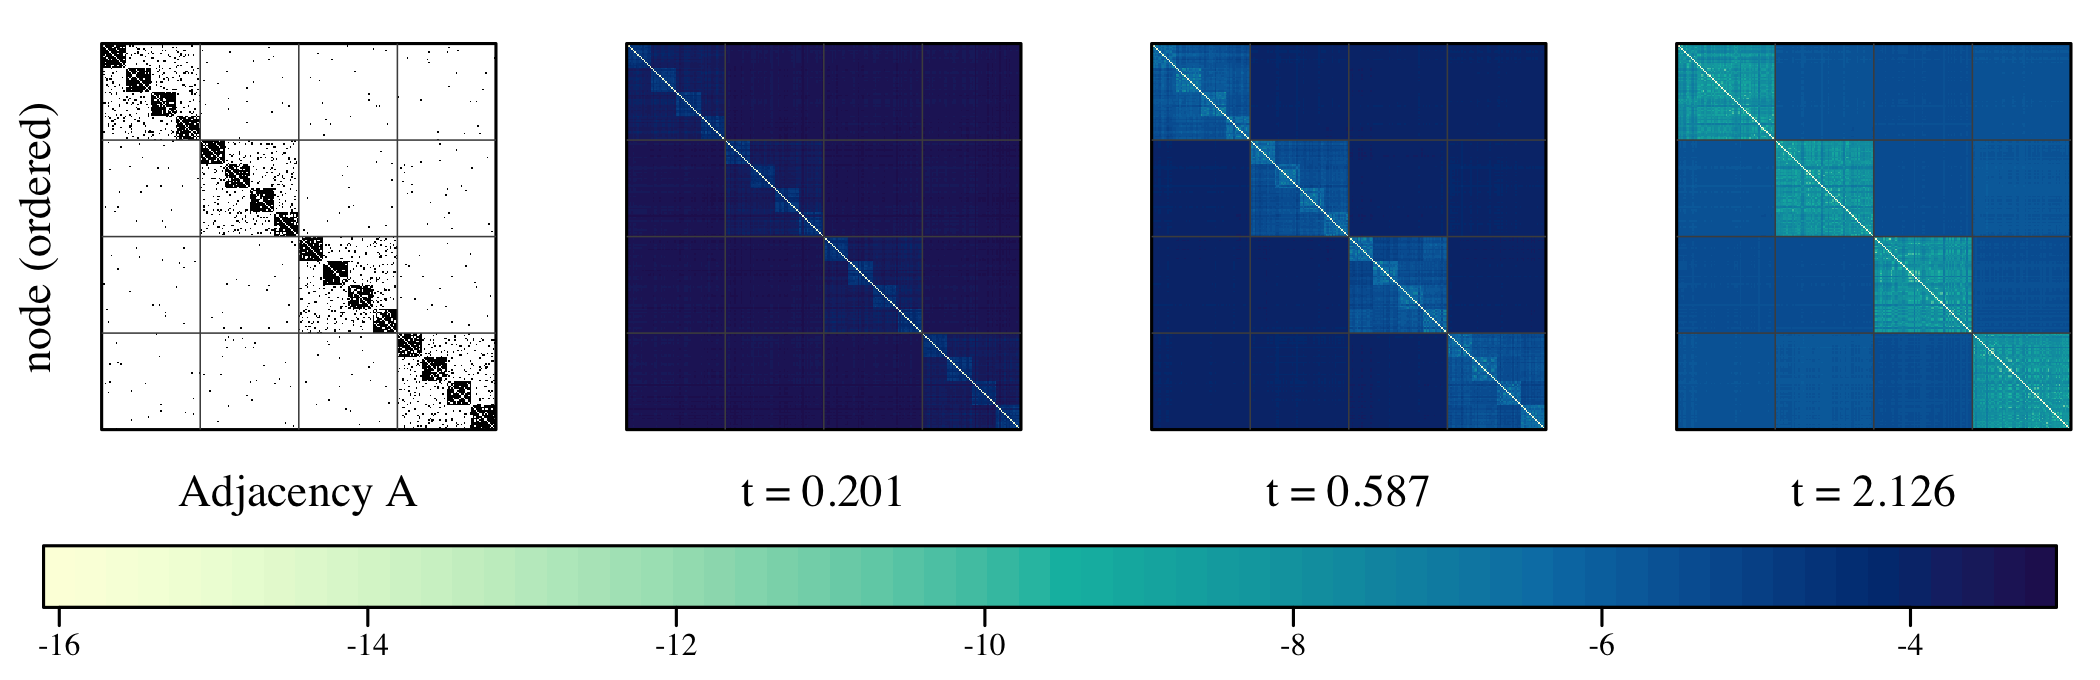
\includegraphics[width=\textwidth]{images/F1_rho_heatmaps.png}
  \caption{\textbf{Adjacency and transient synchronization dissimilarity heatmaps.} Left to right: True adjacency matrix $\mathbf{A}$, and log-dissimilarity $\log_{10}(1 - \rho_{ij}(t))$ evaluated at $t=0.201$ (micro-community sync), $t=0.587$ (meso-community sync), and $t=2.126$ (global sync).}
  \label{fig:rho_heatmaps}
\end{figure}

Figure~\ref{fig:rho_heatmaps} compares the network topology against snapshots of the synchronization dissimilarity $\log_{10}(1 - \rho_{ij}(t))$. Over an ensemble of 100 Runge-Kutta 4 (RK4) realizations of the full non-linear system~\eqref{eq:kuramoto_eq} ($\sigma = 0.4$, $K=1.0$), the pairwise root-mean-square error $\mathrm{RMS}(t) = \frac{1}{N}\sqrt{\sum_{i,j} (\rho_{ij}^{\mathrm{sim}} - \rho_{ij}^{\mathrm{lin}})^2}$ drops below $10^{-4}$ for $t \ge 0.106$ ($\mathrm{RMS} = 7.88 \times 10^{-5}$ at $t=0.106$, and $\mathrm{RMS} = 4.20 \times 10^{-6}$ at $t=0.587$), confirming exact agreement.

\section{Spectral Structure, Null Models, and Participation Ratios}
\label{sec:t6_spectrum}
To discern genuine structural modes from finite-size random graph fluctuations, we construct a degree-preserving null model using Maslov-Sneppen double-edge swaps~\cite{maslov2002} ($n_{\mathrm{swap}} = 20E$).

\begin{figure}[htbp]
  \centering
  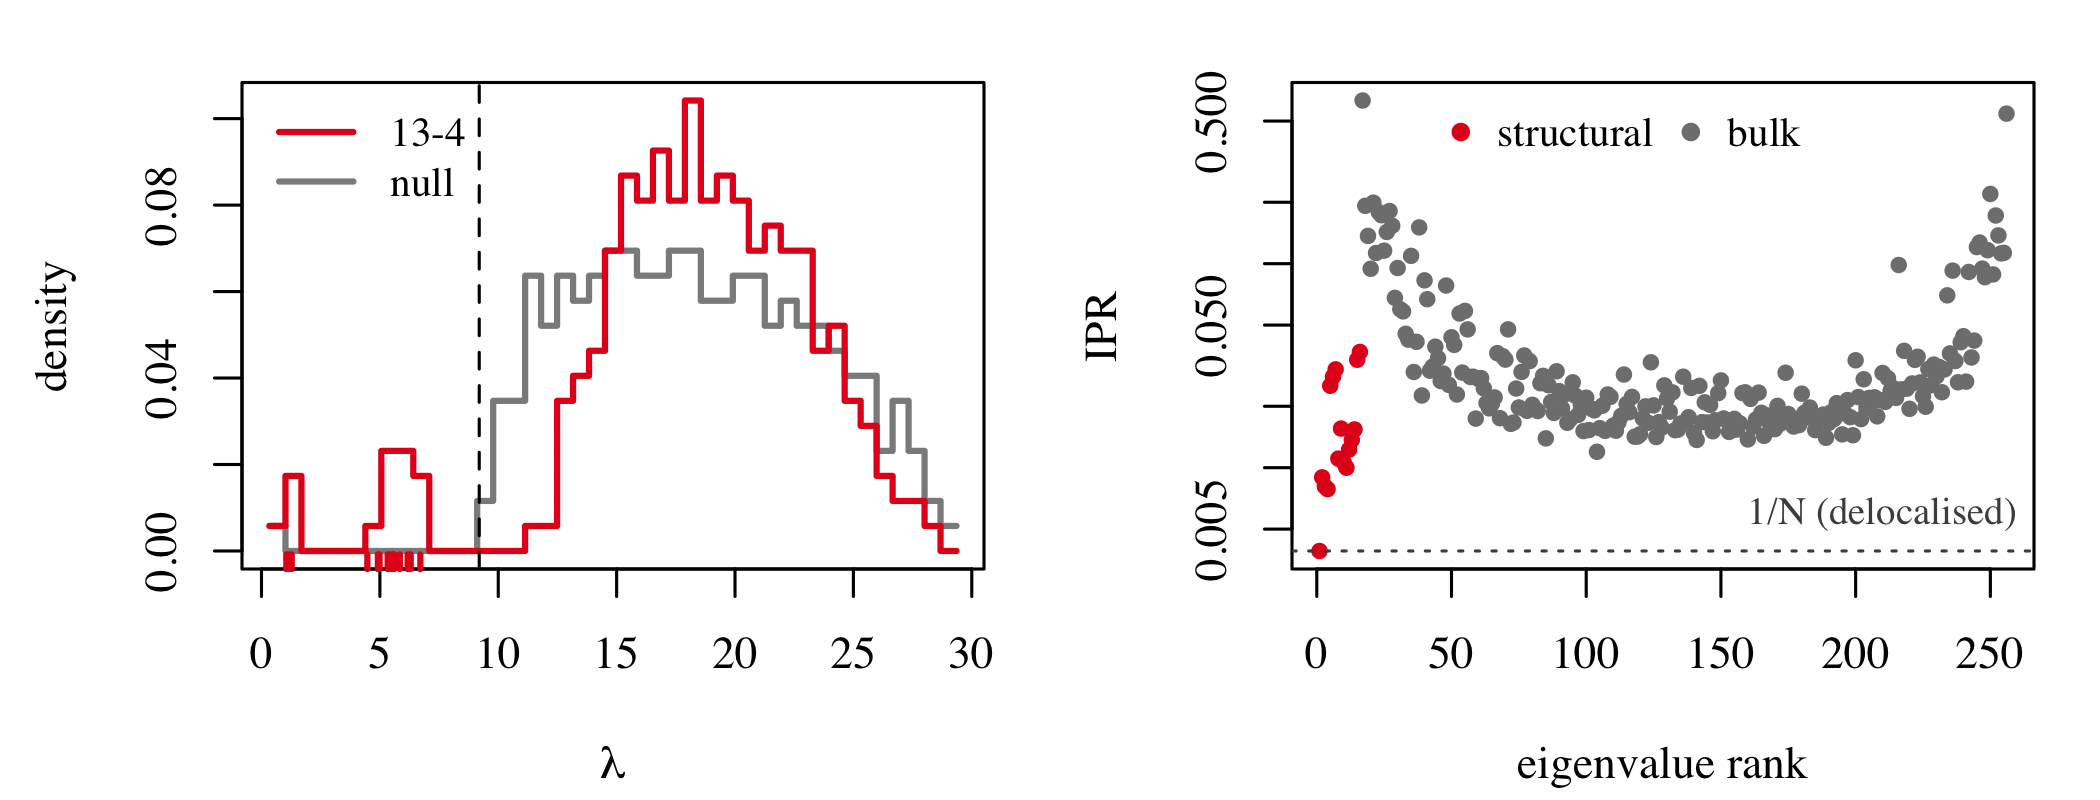
\includegraphics[width=0.98\textwidth]{images/F2_spectrum.png}
  \caption{\textbf{Spectral density and localization of Laplacian eigenmodes.} Left: Spectral density of the 13-4 network (red) compared against the randomized null model (grey) and the bulk edge $\lambda_{\mathrm{bulk}} = 9.20$ (dashed). Right: Inverse Participation Ratio (IPR) across eigenvalues, highlighting delocalized structural modes ($\lambda < \lambda_{\mathrm{bulk}}$, red) versus localized bulk modes (grey).}
  \label{fig:spectrum_null}
\end{figure}

As shown in Figure~\ref{fig:spectrum_null}, the 13-4 network exhibits exactly 16 eigenvalues below the randomized bulk edge ($\lambda_{\mathrm{bulk}} = 9.20$): 3 meso-scale modes ($\lambda_2 = \lambda_3 = \lambda_4 = 1.34$) and 12 micro-scale modes ($\lambda_5 = \dots = \lambda_{16} = 4.88$). Computing the Inverse Participation Ratio $\mathrm{IPR}(\mathbf{v}_\alpha) = \sum_{i=1}^N v_\alpha(i)^4$ confirms that all 16 structural modes are delocalized ($\mathrm{IPR} \approx 1/N$), whereas bulk modes show elevated localization ($\mathrm{IPR} \gg 1/N$).

\begin{figure}[htbp]
  \centering
  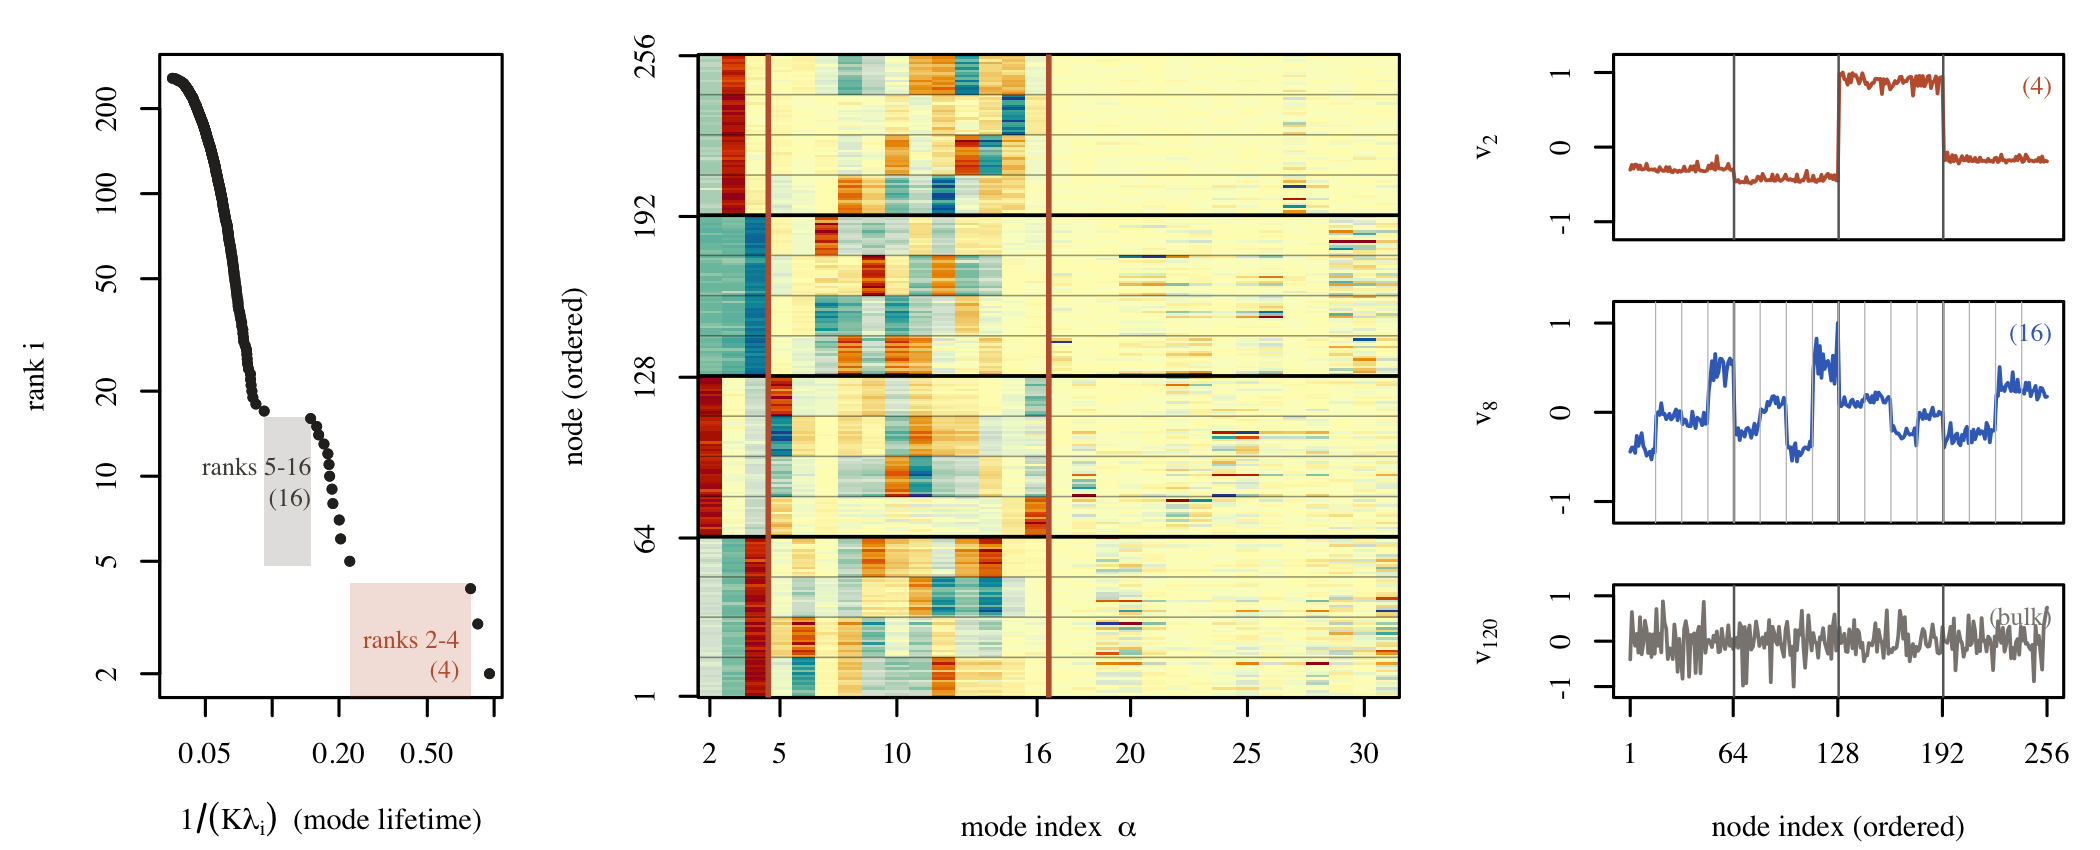
\includegraphics[width=0.98\textwidth]{images/F3_eigenvectors.png}
  \caption{\textbf{Eigenvector profiles and relaxation lifetimes.} Left: Eigenmode lifetimes $\tau_i = 1/(K\lambda_i)$, marking spectral gaps at $m=4$ ($\lambda_5/\lambda_4 = 3.64$) and $m=16$ ($\lambda_{17}/\lambda_{16} = 1.64$). Center: Eigenvector matrix $\mathbf{v}_\alpha(i)$ for modes $\alpha=2..31$. Right: Spatial profiles of modes $v_2$, $v_8$, and bulk mode $v_{120}$.}
  \label{fig:eigenvectors}
\end{figure}

\section{Component Plateaus and Timescale Hierarchy}
\label{sec:t6_plateaus}
A spectral gap $\lambda_m \ll \lambda_{m+1}$ separates modes $\alpha \ge m+1$ that have decayed from modes $\alpha \le m$ that remain active over the temporal window $[ (K\lambda_{m+1})^{-1}, (K\lambda_m)^{-1} ]$. Over this interval, single-linkage clustering (SLINK~\cite{sibson1973}) on $d_t(i,j)$ displays a robust plateau of $m$ disconnected components.

\begin{figure}[htbp]
  \centering
  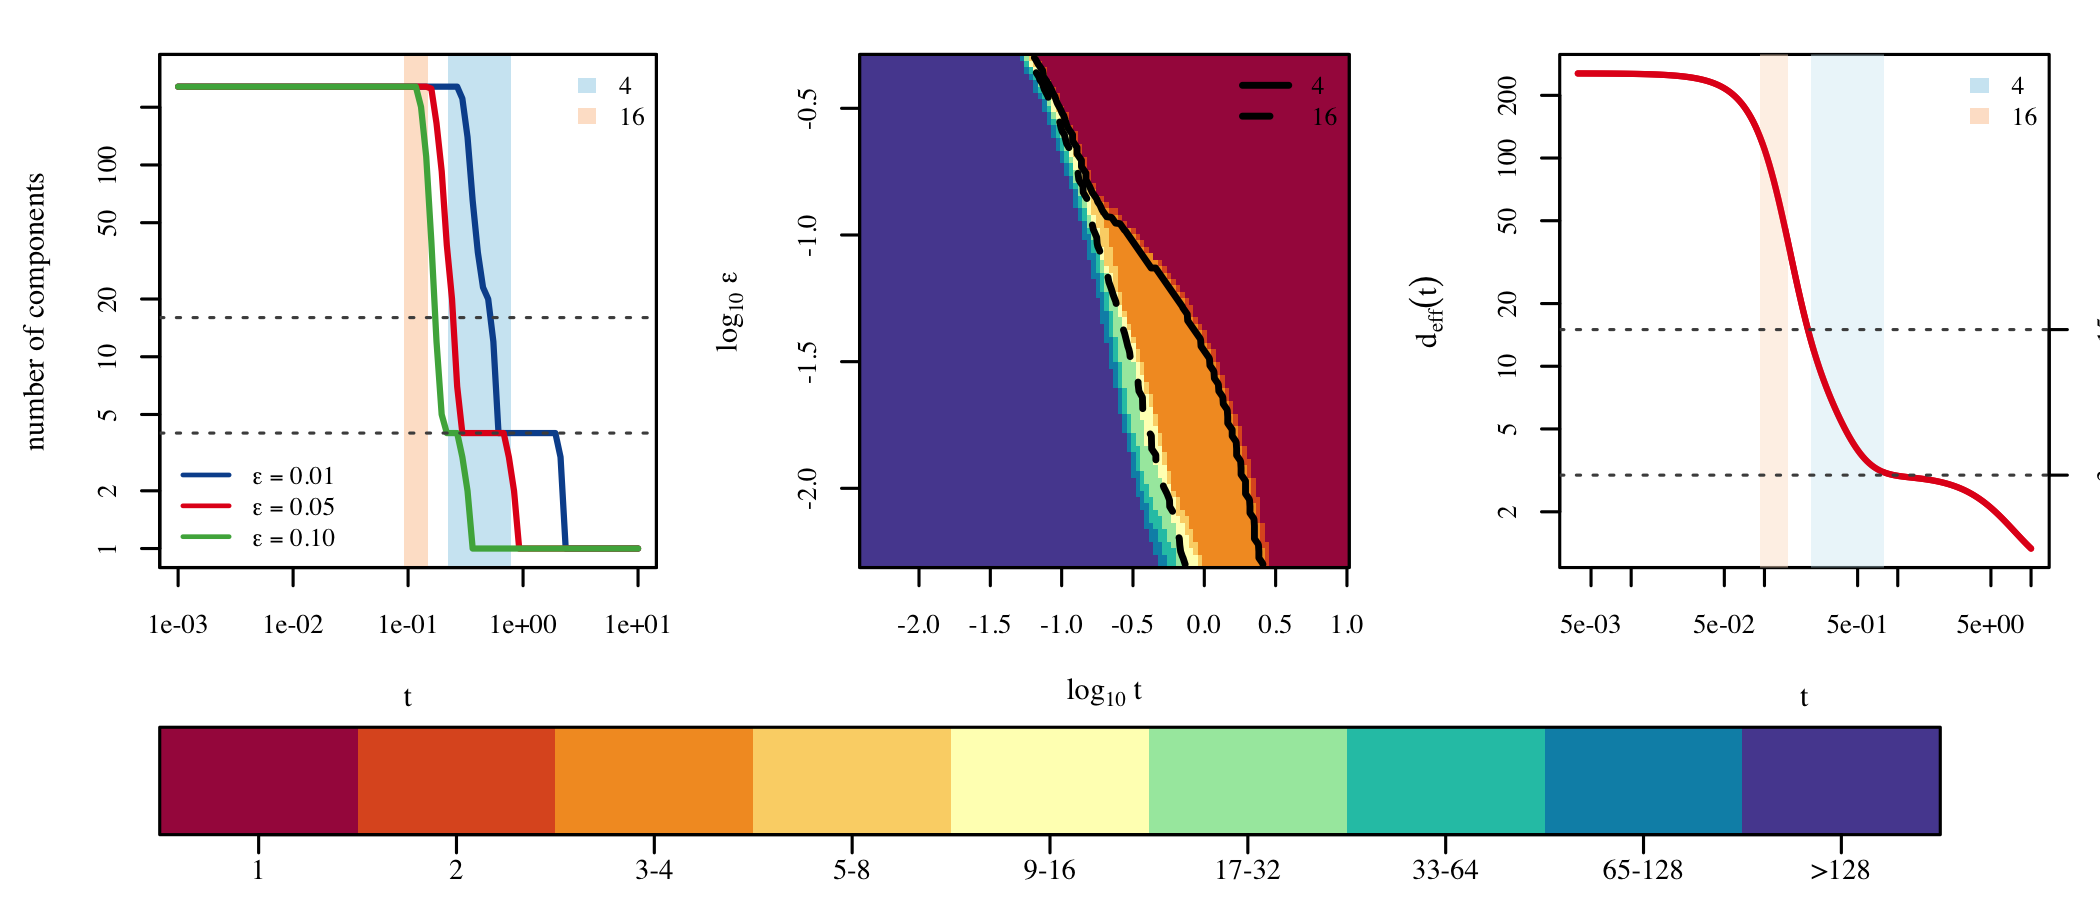
\includegraphics[width=0.98\textwidth]{images/F3_F4_F5_plateaus_geometry.png}
  \caption{\textbf{Plateau dynamics and diffusion embedding geometry.} Left: Number of single-linkage components $n_{\mathrm{comp}}(t)$ showing stable plateaus at 16, 4, and 1 clusters. Center: $(t, T)$ phase diagram where color encodes component count. Right: Diffusion embedding dimension $d_{\mathrm{eff}}(t)$ and pairwise distance spread.}
  \label{fig:plateaus_geometry}
\end{figure}

The predicted plateau length in logarithmic time $\Delta \log_{10} t = \log_{10}(\lambda_{m+1}/\lambda_m)$ agrees with observations (Table~\ref{tab:t6_plateaus}).

\begin{table}[htbp]
\centering
\small
\caption{Spectral gaps and plateau durations for the 13-4 network.}
\label{tab:t6_plateaus}
\begin{tabular}{cccccc}
\toprule
Partition Level & Modes & Gap Ratio $\lambda_{m+1}/\lambda_m$ & Predicted $\Delta \log_{10} t$ & Observed $\Delta \log_{10} t$ & NMI \\
\midrule
4 communities  & $m=4$  & $4.88 / 1.34 = 3.64$ & 0.561 & 0.528 & 1.000 \\
16 communities & $m=16$ & $8.01 / 4.88 = 1.64$ & 0.215 & 0.203 & 1.000 \\
\bottomrule
\end{tabular}
\end{table}

\section{Failure Modes: Hub Contamination and Structural Noise}
\label{sec:t6_failure}
We investigate two critical failure modes of synchronization-based community detection:

\paragraph{1. Degree Heterogeneity (Hubs):} We introduce $n_{\mathrm{hub}} \in [1, 8]$ hubs connected uniformly across modules. Adding 8 hubs ($\sim 3\%$ of nodes) completely destroys the 4-community plateau (Figure~\ref{fig:hubs_failure}). In diffusion space, hubs collapse to the diffusion centroid ($\|\mathbf{\Psi}_t(h)\| \approx 0$), acting as topological shortcuts that artificially merge clusters prematurely.

\begin{figure}[htbp]
  \centering
  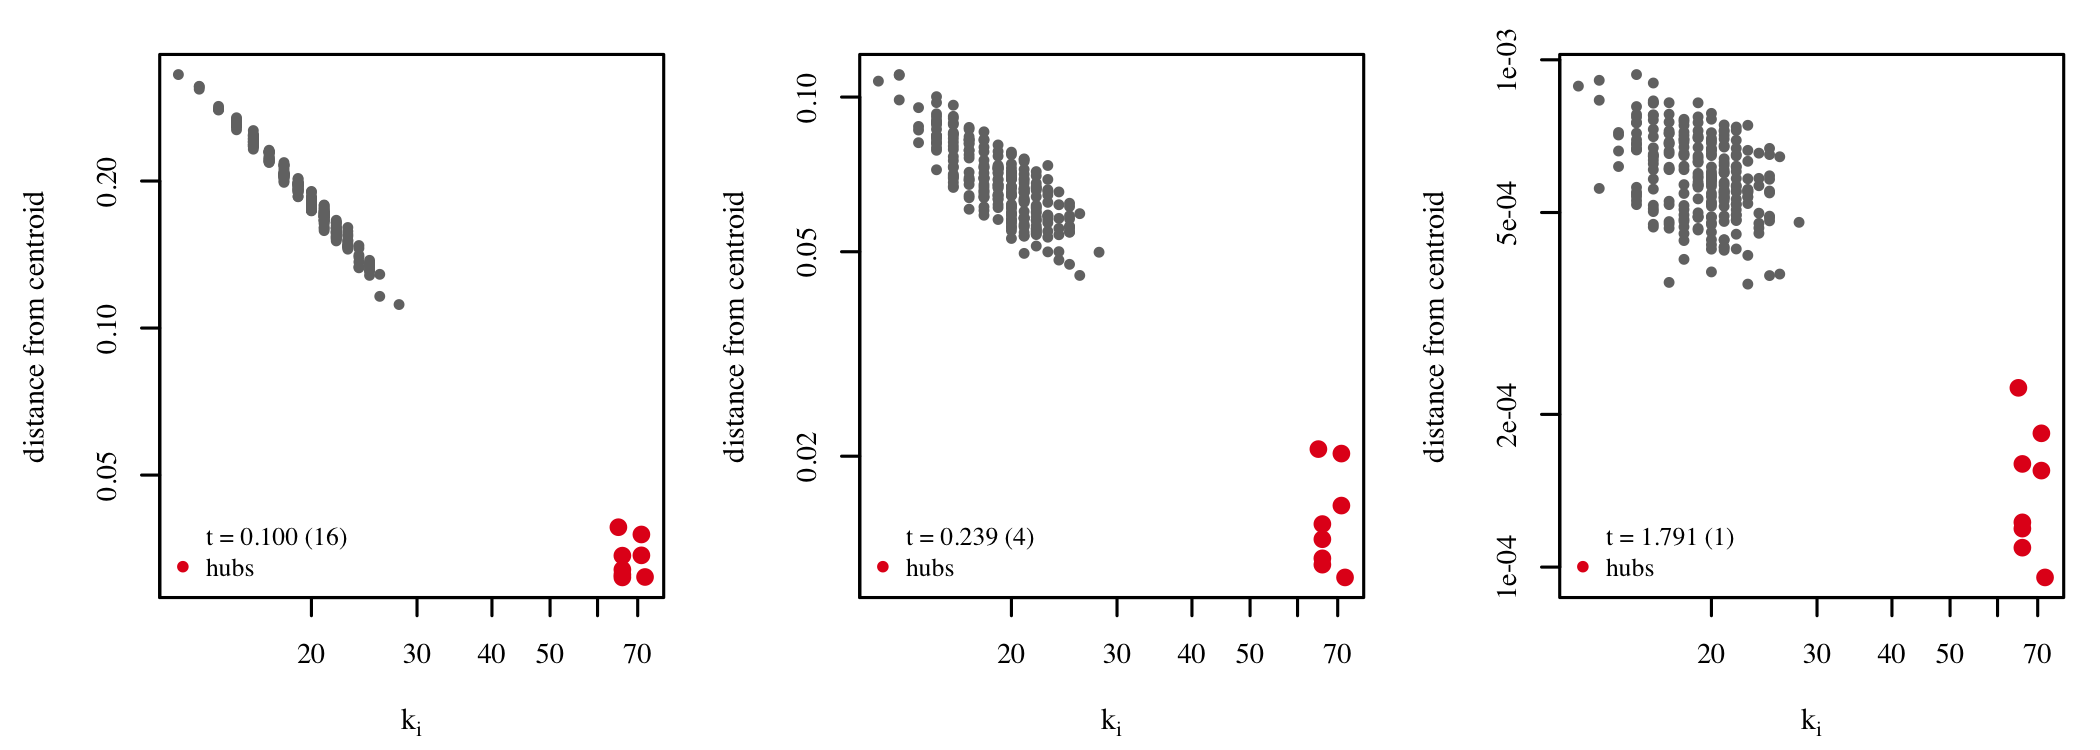
\includegraphics[width=0.48\textwidth]{images/F6_hubs_test.png}
  \hfill
  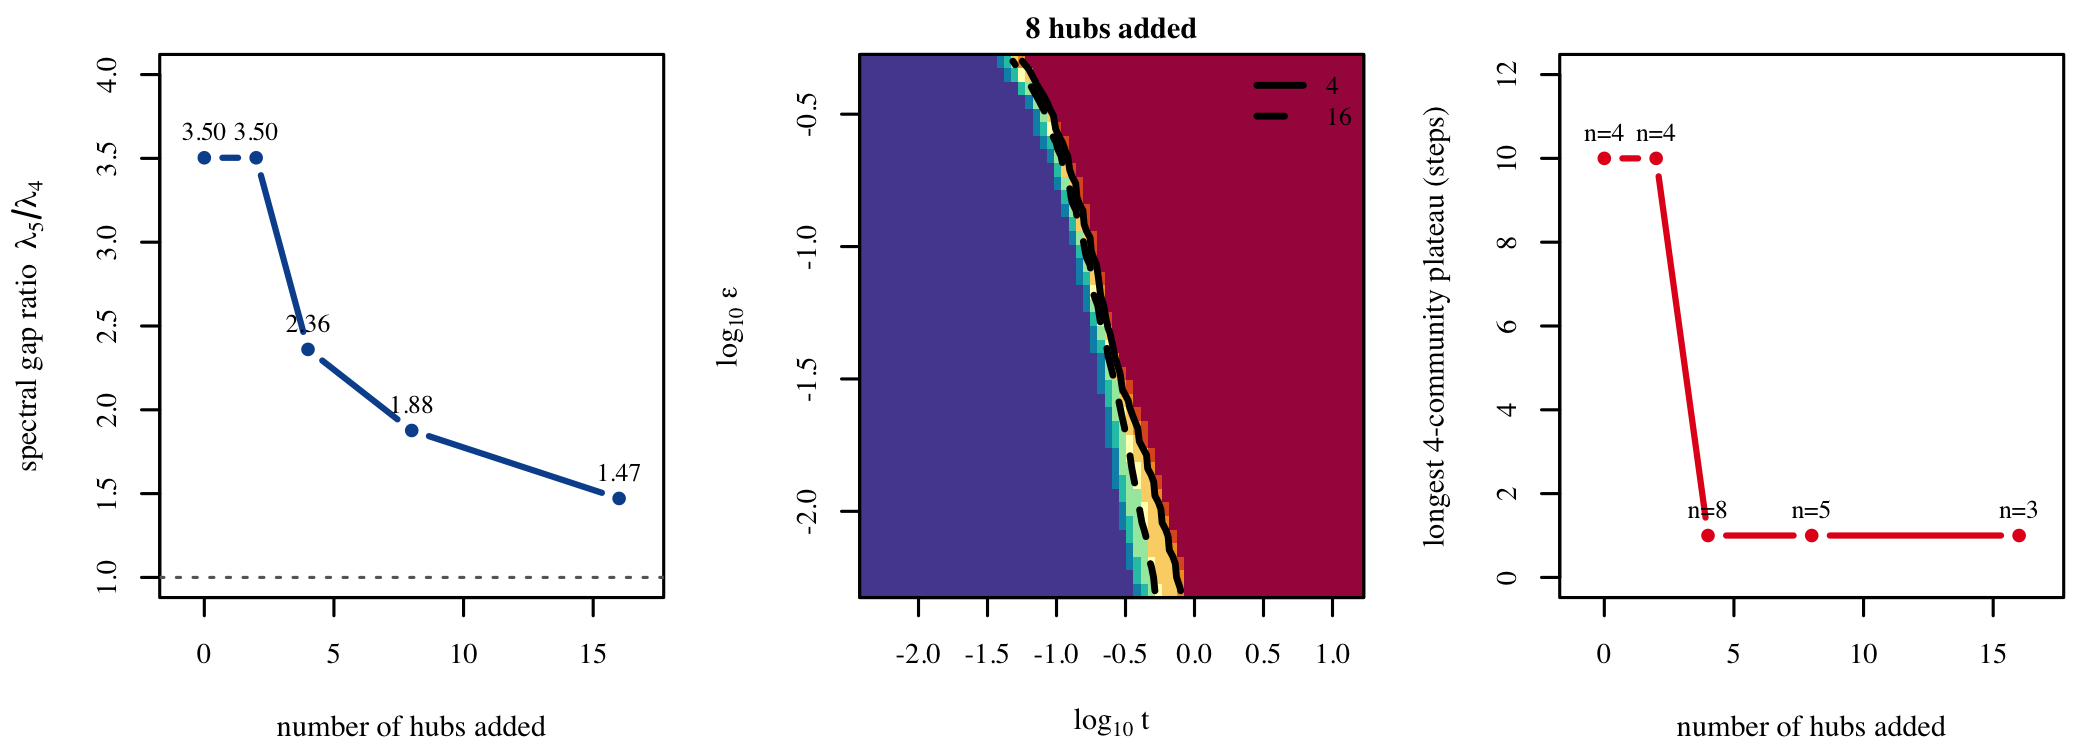
\includegraphics[width=0.48\textwidth]{images/F7_hub_damage.png}
  \caption{\textbf{Degradation induced by targeted hub contamination.} Left: $(t, T)$ plane with 8 hubs added, showing complete destruction of the $m=4$ plateau. Right: Plateau duration and algebraic connectivity as a function of hub count.}
  \label{fig:hubs_failure}
\end{figure}

\paragraph{2. Structural Noise Sweep ($z_{\mathrm{out}}$):} Increasing $z_{\mathrm{out}} \in [1, 14]$ while keeping $\langle k \rangle = 18$ fixed shrinks the spectral gap $\lambda_5/\lambda_4$. Notably, plateau visibility vanishes at $z_{\mathrm{out}} \approx 6$, well before static NMI recovery degrades at $z_{\mathrm{out}} \approx 11$ (Figure~\ref{fig:zout_sweep}). Thus, the regime where synchronization dynamics reveals topological scales via plateaus is strictly narrower than the statistical detectability threshold.

\begin{figure}[htbp]
  \centering
  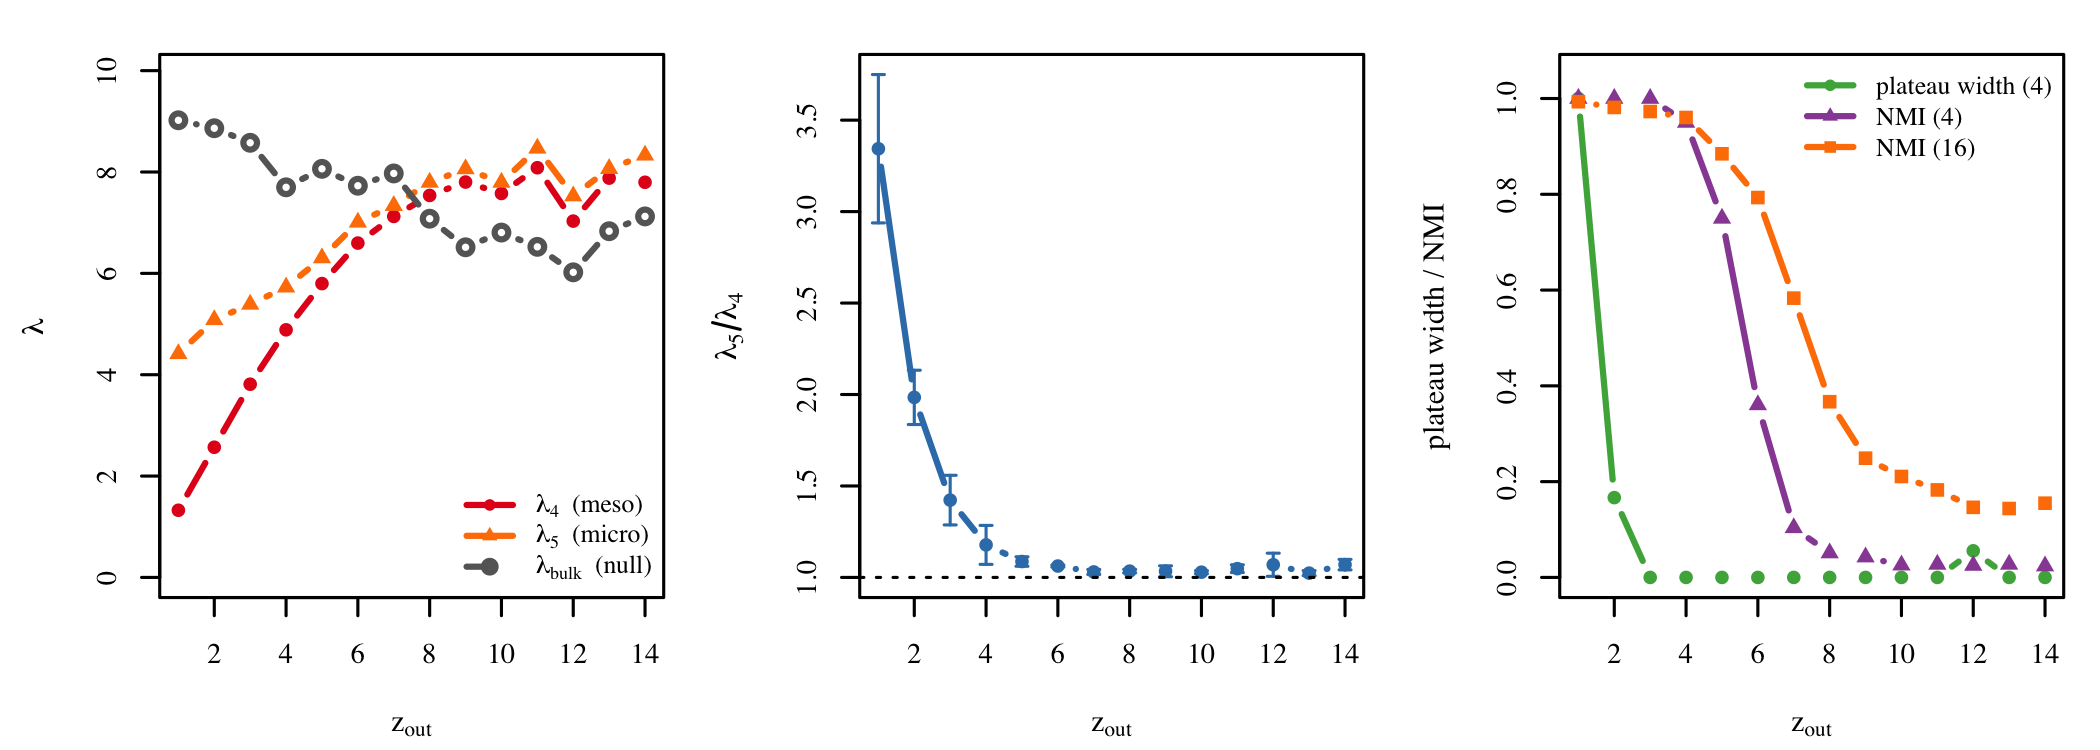
\includegraphics[width=0.98\textwidth]{images/F8_zout_sweep.png}
  \caption{\textbf{Robustness sweep over inter-community degree $z_{\mathrm{out}}$.} Left: Eigenvalues $\lambda_4$ and $\lambda_5$ relative to bulk edge $\lambda_{\mathrm{bulk}}$. Center: Spectral gap ratio $\lambda_5/\lambda_4$. Right: Normalized plateau width versus static NMI recovery.}
  \label{fig:zout_sweep}
\end{figure}

\section{Reproducibility, Repository, and AI Use Disclaimer}
\label{sec:t6_repro}
Source code, data, and scripts for Task 6 are available in the public repository:
\begin{center}
\url{https://github.com/filippobezzi/PoCN_projects}
\end{center}

\paragraph{AI Assistance Disclaimer:}
The author acknowledges the use of generative artificial intelligence assistance (DeepMind's Antigravity AI assistant) for writing assistance, code development, data formatting, and proofreading the manuscript. All analytical derivations, mathematical proofs, numerical simulations, and physical interpretations have been rigorously verified by the author.
